\section{Theory}

\subsection{How does Augmented Reality work?}
There are different types of augmented reality. Some of those are marker-based, location-based, superimposition-based and projection-based. \\

\textbf{Marker-based} AR is when markers, in the form of images have to be placed in the real world and detected by the application. Virtual object are rendered on top of these markers. An example would be a picture in a magazine which, when pointing a camera at it, the application renders an 3D object on top.\\

\begin{figure}[hbtp]
\begin{center}
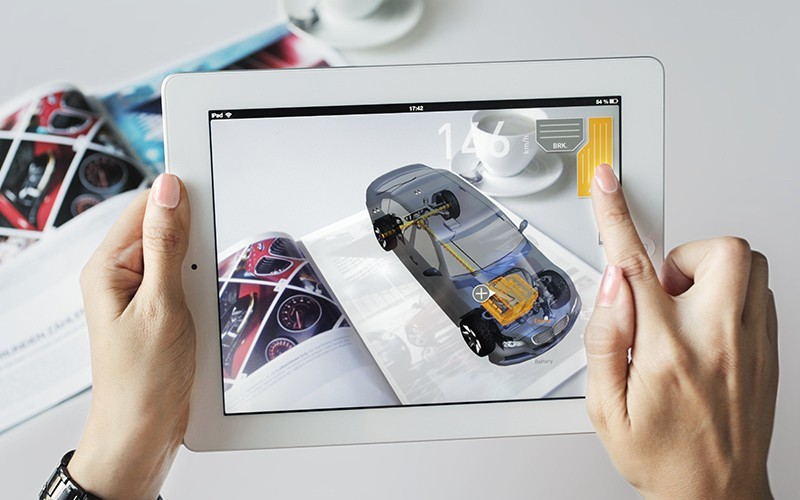
\includegraphics[width = 0.75\textwidth]{./Images/markerbasedar.jpg} 
\caption{A virtual object in the form of a car being rendered on top of a marker in a magazine.}
\end{center}
\end{figure}

\textbf{Location-based} AR is when the content on the users screen differs depending on the location of the user. This type is highly dependent on the GPS signal.
An example of where this could be useful is in a museum where different information could be given to the user depending on which room he is in.\\

\textbf{Superimposition-based} AR uses object recognition in order to enhance that object with some sort of visual information. It replaces the real object with an enhanced virtual one. It could be used in retail to display different patterns on a piece of clothing.\\

\textbf{Projection-based} AR is when virtual object can be placed in a room to make it appear as if they were there. A popular example of this would be the IKEA Place app that was mentioned in the introduction.  \\

\begin{figure}[hbtp]
\begin{center}
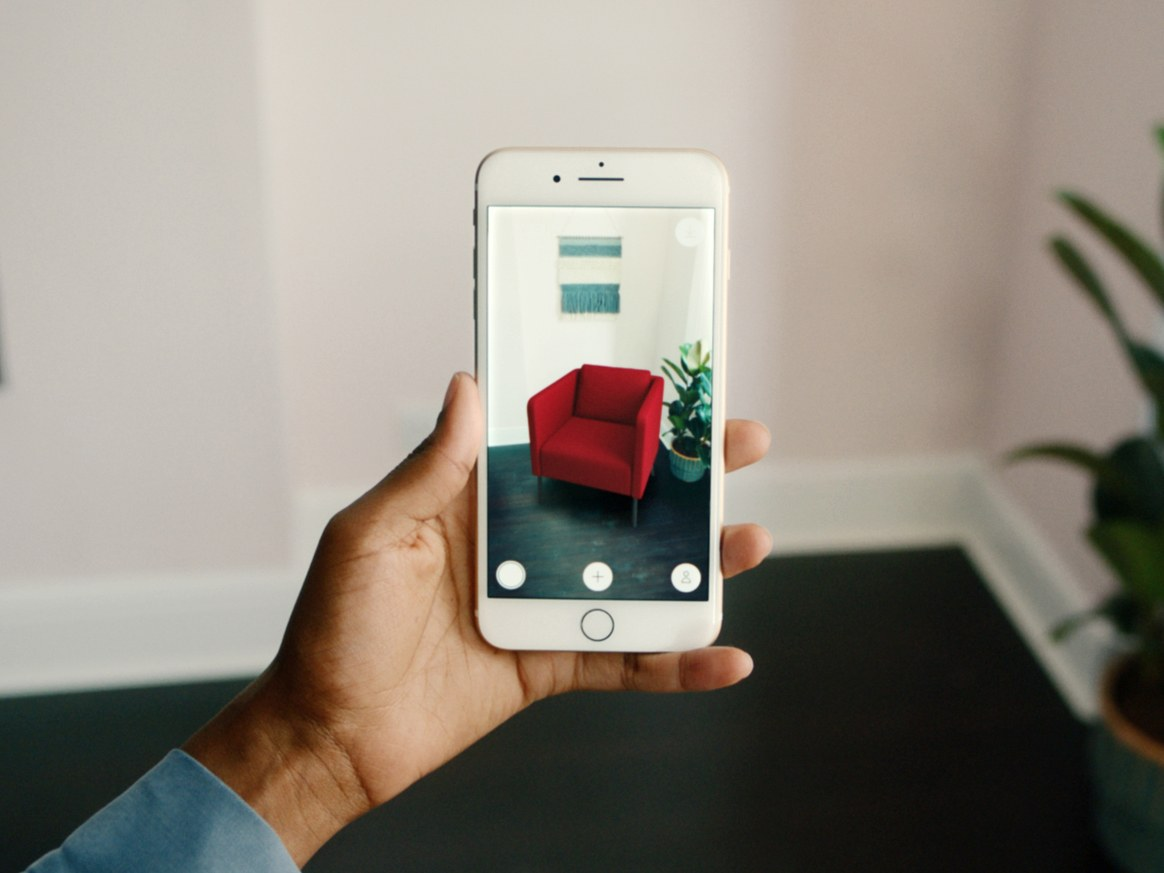
\includegraphics[width = 0.75\textwidth]{./Images/ikeaplace.jpg} 
\caption{A virtual sofa chair being added to a room within the IKEA Place app.}
\end{center}
\end{figure}

In this paper we will mainly be using projection based AR with a form of recognition. The projections will be in the form of way-pointers used as instructions for the user to perform the next step in putting together a furniture piece. These instructions can visualize how the pieces will look like after the step is completed, and to show arrow pointers between the pieces that are supposed to be put together.

\subsubsection{History of AR}
The idea of augmented reality has existed a long time, the phrase has only been used for about 28 years but it is not until recently that the technology has become mainstream.
This is mainly due to it becoming good enough to be used by the average person at home. Today we can just download an app on our smart phones to enjoy the technology. Below follows a brief history of how augmented reality has progressed throughout the years.\\

\textbf{1968}
The Sword of Damocles - The first mounted headset.
This device was mounted on the head and could display a cube wireframe floating in the air. It was invented by Ivan Sutherland.\\

\textbf{1975}
Myron Krueger - Videoplace. Using cameras to interact with a digital world with shadows.
This application could be used to draw things or play simple video games with the shadow of your hand.
\cite{videoplace}\\

\textbf{1990}
The first time the term "Augmented Reality" was used by the Boeing researcher Tom Caudell.\\

\textbf{2009}
AR comes to the web in the form of an open source toolkit called ARToolKit.\\

\textbf{2017}
Apple launches AR Kit and Google launches AR Core.\\

\subsubsection{S.L.A.M.}
S.L.A.M (Simultaneous Localization and Mapping) is a way for a machine to get to know the environment that it is in. It registers features and maps them to its surroundings. S.L.A.M is about having the map of the environment and knowing where the robot is in that map.
The problem with this is that a map is needed for knowing where you are, and you have to know where you are to be able to create a map. That is why S.L.A.M is doing this at the same time, hence 'Simultaneous'. The system is used in autonomous robots, but also valuable in Augmented Reality. \cite{slam}

iPhone X does this by tracking multiple reference points in space and from them building a 3D model of the surroundings using a form of S.L.A.M technique.
This is accomplished by keeping a map of the features while keeping track of the path the observer is taking. A number of 
hardware components make this task possible, including gyro, accelerometer and a compass. \cite{iphoneslam}

\begin{figure}[hbtp]
\begin{center}
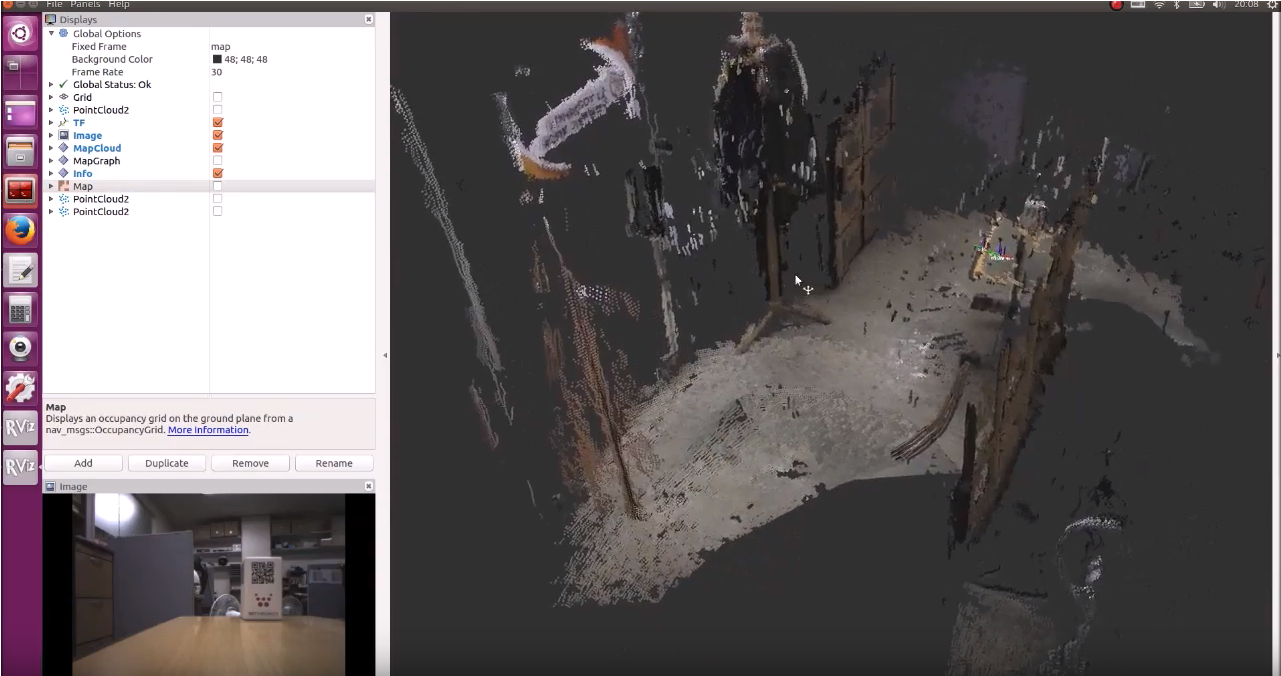
\includegraphics[width = 0.75\textwidth]{./Images/slam-map.jpg} 
\caption{A robot performing S.L.A.M in an environment and the 3D model created.}
\end{center}
\end{figure}

\subsubsection{Other inputs}
Compass, Gyroscope, Accelerometer  etc.

\subsubsection{How does ARKit work?}
ARKit works similar to SceneKit were a scene (which is basically a 3D environment in which nodes containing 3D models (geometry) can be rendered) is loaded at start up and interacted with.
An ARScene is contained inside an ARSCNView (AR Scene View) which also has a ARSession
that that manages the motion tracking and camera image processing. For an ARScene to work, it must have a running ARSession.
The session is started with configuration (ARConfiguration). This configuration can be of many kinds, the most common ones begin ARWorldTrackingConfiguration and ARFaceTrackingConfigurations. For this project, ARWorldTrackingConfiguration will be used since the face tracking one uses the front camera.

Below, an example of how to setup a configuration and running a session is given:

\lstinputlisting[language=swift,firstline=55,lastline=74]{../../Application/ObjectDetectionInAR/ObjectDetectionInAR/Assembler/AssemblerViewController.swift}

But before a session can be started, an ARScene must exists and be loaded. The ARScene is a regular .scn file that has the starting nodes that together form the starting
environment the user will interact with. An example of how a scene like that looks like is shown in figure \ref{fig:3dsceneImage}.

\begin{figure}[hbtp]
\begin{center}
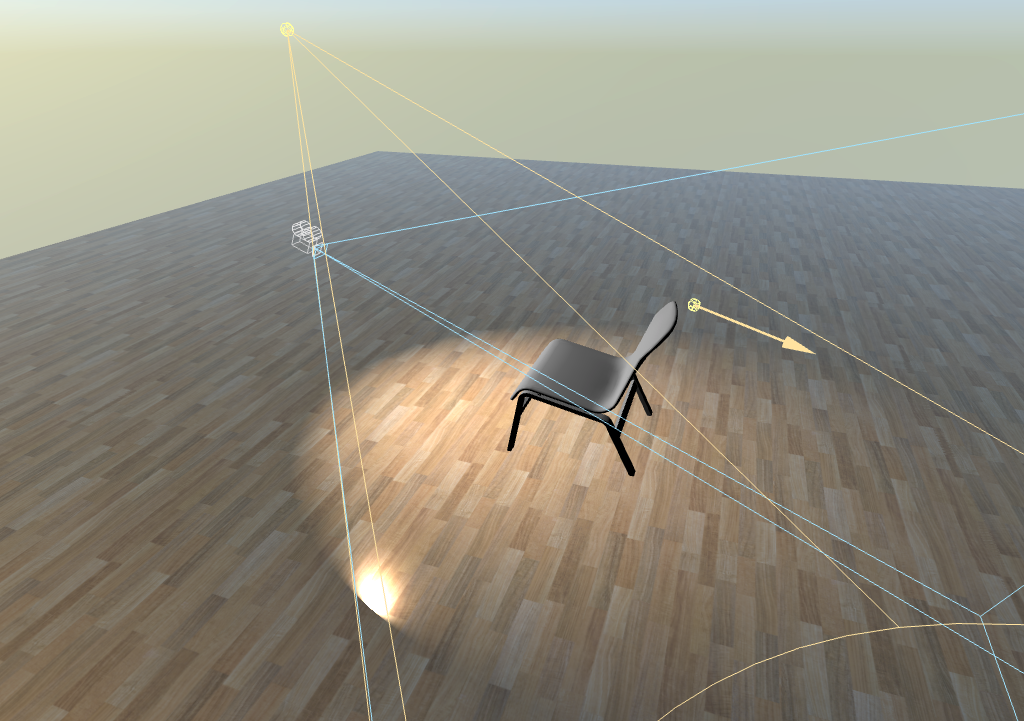
\includegraphics[width = 0.75\textwidth]{./Images/3dscene.jpg} 
\caption{An example of a 3D scene created in XCode with a camera, a plane, directional light and three geometry nodes.}
\label{fig:3dsceneImage}
\end{center}
\end{figure}

To load a scene, a new .scn file must be created in the art.scnassets folder and fetched like below.
\lstinputlisting[language=swift,firstline=154,lastline=156]{../../Application/ObjectDetectionInAR/ObjectDetectionInAR/Assembler/AssemblerViewController.swift}

When ARScene detects objects, images, planes etc. it calls the renderer function. This function can be implemented by setting the ViewController to conform to the ARSCNViewDelegate. ARScene adds an anchor (ARAnchor) and a node (SCNNode) for the place where it detected it, and this can be used inside the function to render new nodes or other logic.

\lstinputlisting[language=swift,firstline=215,lastline=230]{../../Application/ObjectDetectionInAR/ObjectDetectionInAR/Assembler/AssemblerViewController.swift}

If nodes need to be rendered outside of this function it can be done by accessing the
scenes root node.

\lstinputlisting[language=swift,firstline=105,lastline=105]{../../Application/ObjectDetectionInAR/ObjectDetectionInAR/Assembler/AssemblerViewController.swift}

\subsection{What Machine Learning methods are there?}
There exists many different machine learning techniques out there today. Due to its high effectiveness and relevance, for this report we are going to focus on the highly popular method of artificial neural networks.
This is a proven method for working well with images (Convolutional neural networks) and is therefore a highly 
relevant technique for this project.

\subsubsection{Perceptron}
A perceptron is the simplest form of the neural network. It has a set of inputs and an output.
The perceptron first sums up all the input values, x, multiplied with the weight value, w.
After that it passes that sum through an activation function. This activation function can be everything from a simple f(x)=x to the more complex sigmoid function, depending on the need. More on this in the upcoming section.

\begin{figure}[hbtp]
\begin{center}
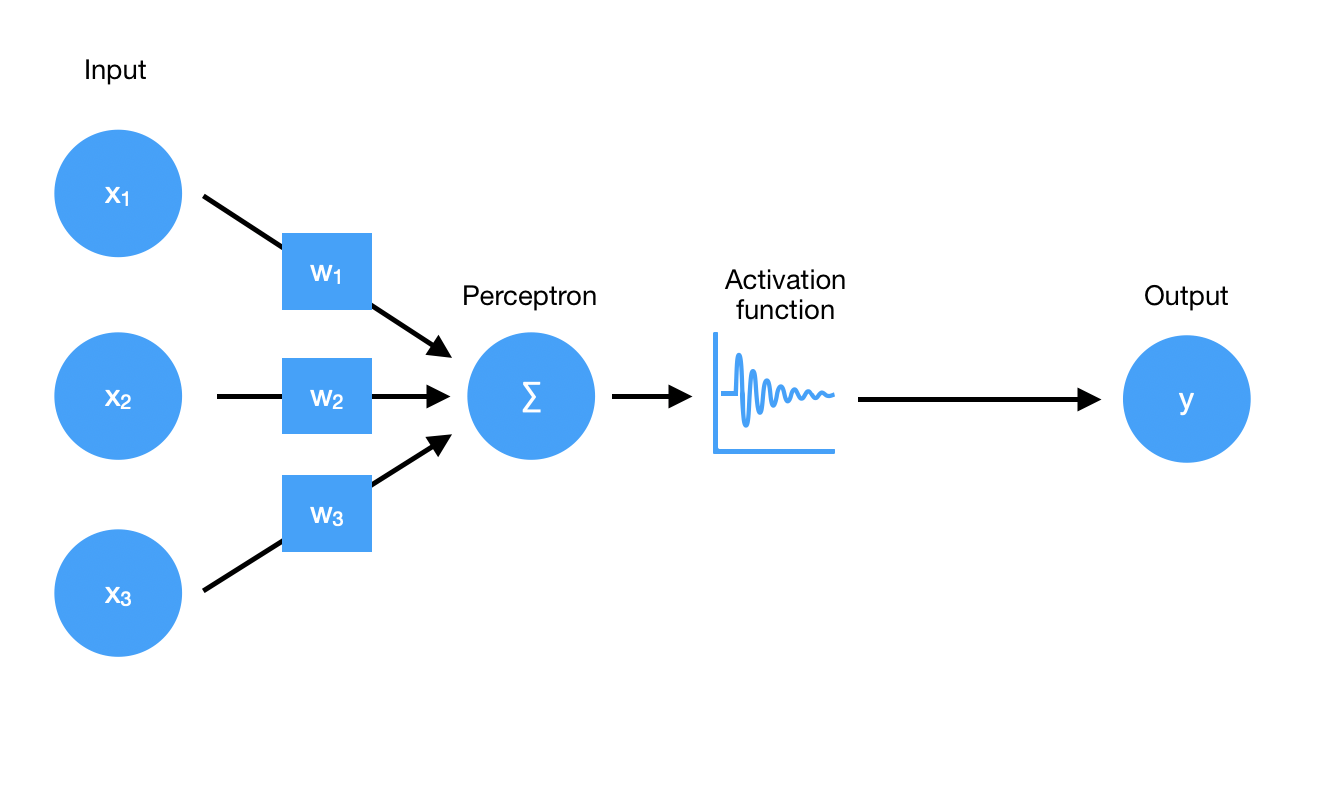
\includegraphics[width = 0.75\textwidth]{./Images/perceptron.jpg} 
\caption{An illustration of the perceptron, the simplest version of a neural network.}
\end{center}
\end{figure}

A bias also exists in every node which is not based on any input. The bias function in the perceptron is similar to what the m in $y = kx + m$ does. It gives the function the ability to move up and down in the graph for more possibilities of splitting the data set. The bias is usually disregarded when illustrating the perceptron.

The perceptron only has the ability to draw a single line and thus is only able to split simple data sets.

The output of the perceptron is described by the following formula:

\[ y = b + \displaystyle\sum_{i=1}^{n} x_i \cdot w_i \]

where b is the bias value, x is the input, w is the weight for that input and n is the number of inputs.

\subsubsection{Activation functions}

The activation function,  $ \phi (v_{i}) $ , takes the sum of all the inputs from a node as input and passes them through a function before giving an output. This is beneficial when for instance the output should be kept in a range between 0 and 1, or perhaps when negative values don't make sense.
Usually, activation functions are attributed to layers instead of individual nodes.

The most common of these functions are \textbf{ReLu}, \textbf{Tanh}, \textbf{Sigmoid} and \textbf{Softmax}.

\textbf{ReLu} is described as
\[f(x) = max(0, x)\]
and is a good option when negative values should be ignored or don't make sense. Problems with ReLu?

\textbf{Tanh} is the tangens hyperbolicus function and is used to output values either as -1 or 1 like a binary operator. Unlke a binary operator, tanh's derivative is always defined which makes back propagation possible.

\textbf{Sigmoid} is described as 
\[\frac{e^x}{1+e^x}\]
and works like the Tanh function but keeps the values between 0 and 1 and sets y(0) = 0.5 instead.

\textbf{Softmax} is a little bit more complex. It takes a vector $v$ of dimension $n$ and turns it into a vector $\sigma(v)$ of the same dimension where $\displaystyle\sum_{i=1}^{n} \sigma_i(v) = 1 $ and each element value is between zero and one.

Each element in the array is described as below
\[ \sigma_i(v) = \frac{e^{v_i}}{\displaystyle\sum_{j=1}^{n} e^{z_k}} \]

This output is good for describing the probability for each element to be correct and is therefore commonly used
in the output layer.

\subsubsection{Loss/Optimizers}
When training the model using backpropagation, the model will at first make a guess to what the right answer or value is based on the random initial weigh values. In the beginning, the model is usually mostly wrong and it is then important to know how wrong it was and in what direction it should go.

For this, the model uses a loss function to calculate that error. For different applications the loss function can be different.
One way to calculate the error is to simply take the predicted value and subtract it with the correct value, $ error = y_p - y_c $.

Sometimes the sign of the error is not important. Then the absolute error can be calculated instead. $error = |y_p - y_c| $

Another approach is the \textbf{mean squared error} which squares the difference and takes the mean value over a few predictions.
\[Error = \frac{1}{n} \cdot \displaystyle\sum_{i=1}^{n} (y_p - y_c)^{2} \]

SGD
Adam
Nadam

\subsubsection{Layers}

\begin{figure}[hbtp]
\begin{center}
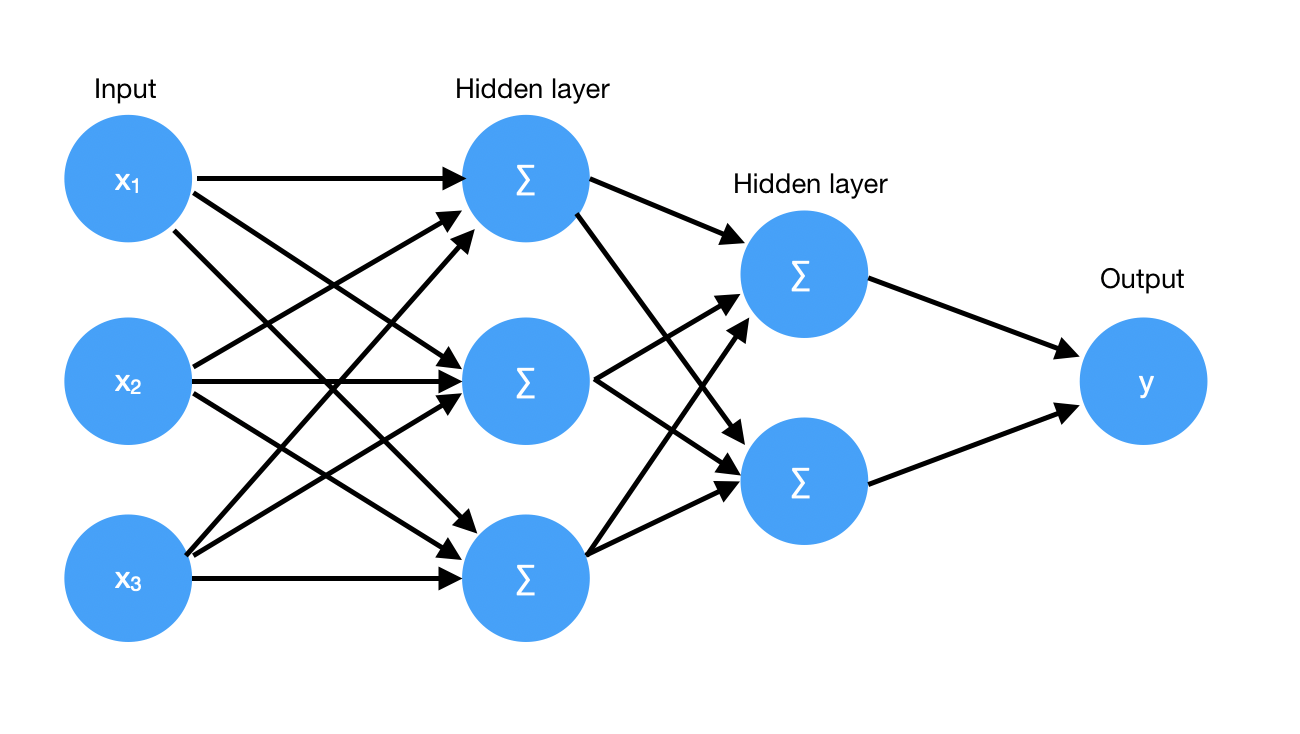
\includegraphics[width = 1.0\textwidth]{./Images/fully_connected.jpg} 
\caption{Two fully connected layers. One with 3 neurons and one with 2 neurons.}
\end{center}
\end{figure}

With more layers and more neurons the networks parameters and complexity begins to grow. So does also the training time, size of the model and the cost for doing predictions. Thus, these networks are capable of describing much more complex data sets. But as a result of that, the risk of overfitting (The act of describing the training data set too well so that new data sets will not get recognized. More on this soon.) becomes much greater. That is why a complex network is not always wanted.

\subsubsection{Overfitting}
When training a neural net, one needs to be careful not to train the model too much or overfitting is likely to happen. Overfitting is when a model gets REALLY good at predicting the data that it is training on but fails to predict accurately on new data. This is because it starts to pick up too much on detail or in some instances even noise. For this reason it fails to pick up the general trends, which is more valuable. 

\begin{figure}[hbtp]
\begin{center}
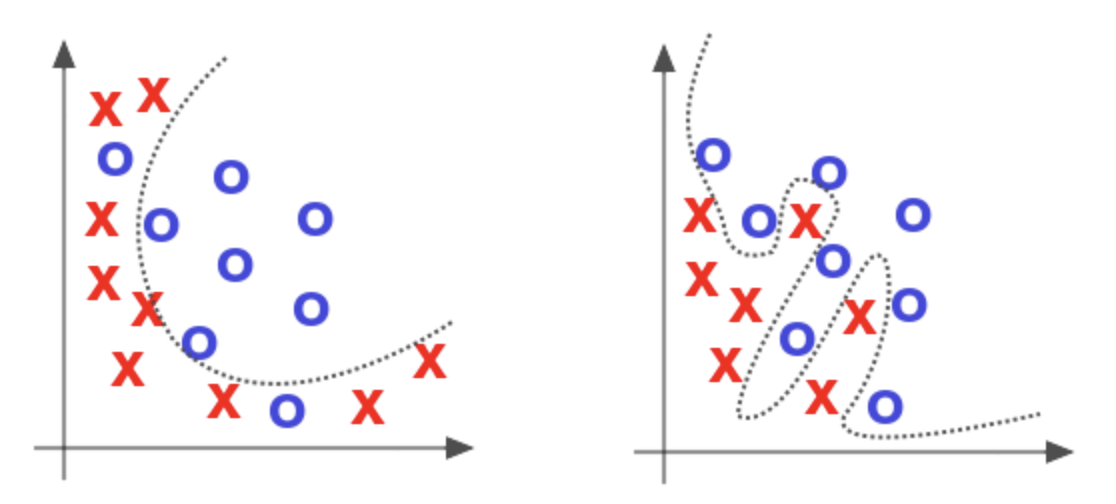
\includegraphics[width = 1.0\textwidth]{./Images/overfitting.jpg} 
\caption{Overfitting of a dataset. On the left is a accurate trained model, on the right is an overtrained model. Image taken from OReilly.com}
\end{center}
\end{figure}

\cite{overfitting}

There are tricks for combating overfitting. They usually involve trying to limit the size of a small amount of weights.
The hypothesis behind this is that if a weight is much larger than the rest it also has much more influence over the final prediction. That way, a small detail in the data can have much more influence than the general trend.

One way to do this is to cut random connections between layers during epochs, usually by specifying a certain amount that is going to be cut.
This way, the model is not relying on a small number of nodes to make the correct predictions. This method is called dropout.

Another way is to introduce random noise on a layer during training. This works because if a node with a large weight receives noise, it will be heavily amplified and probably give a false prediction.
When doing this, Gaussian noise is usually implemented, which is basically random noise with a gaussian distribution.

To force the model to keep weights small, one way is to add a penalty to the loss for every weight based on its size. 
This is called weight regularisation and is widely used and exists in two forms, L1 and L2.
L1 simply adds the weights size multiplied with an l1 term that is chosen by the designer.
The other, L2, is to do the same but in this case square that value. This has the effect of making values over 1 even bigger and values less than 1 smaller.
In that way, it doesn't affect the loss as much as L1 when not being overtrained. L2 is also called weight decay and is the more common method of the two.

Another way to keep the values between 0 and 1 is to normalize the input to every layer. In Tensorflow, this can be done with the BatchNormalization layer.

One important thing to point out is that all these methods mentioned so far are only active during training and is not doing anything when making real predictions.


If lots of training data exists, the ensemble technique could be a good way to go. This technique divides the training data into more smaller sets and trains a model for every data set.
The final prediction is then an average of the predictions of all the models. This technique works because if the model is highly overtrained in a certain direction, chances are that the other networks will drown out this result by the many other models.

It is kind of like when someone has an off pitch in a big choir. If there are many other singers, this off-pitch will not be noticed very much.

\begin{figure}[hbtp]
\begin{center}
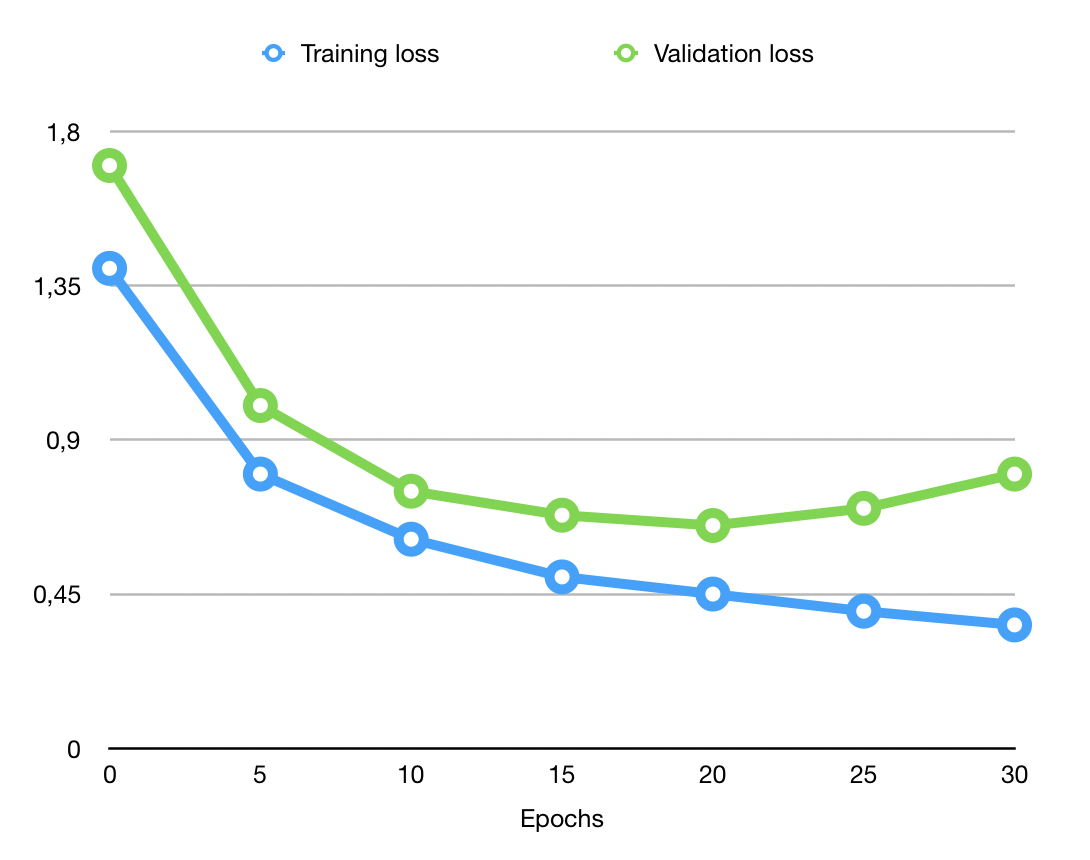
\includegraphics[width = 0.75\textwidth]{./Images/early_stop.jpg} 
\caption{A graph showing when to do an early stop. The graph shows the total loss over trained epochs. Notice that the validation starts to increase again somewhere after epoch 20.}
\end{center}
\end{figure}

The final technique is called early stopping and is based on validating the model after every epoch and stopping the training when the validation loss, or some other criteria, is not improving anymore.

\subsection{Object Detection with traditional machine learning}
% Write about feature based detection and segmentation

When trying to detect objects in a still image we have looked into two main methods. One typical way is to try and look for patterns or features in the image.
Either a specific image can be matched within the larger image or a series of features can be found.
An example of the latter is Haar features which is used in the Viola-Jones for face detection. Using the image integral (which is the summation of pixel values in a specific region) different features can be obtained.

\begin{figure}[hbtp]
\begin{center}
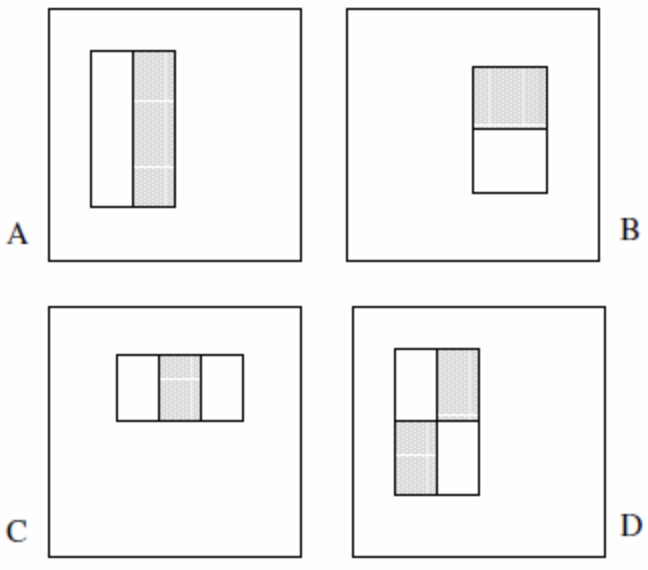
\includegraphics[width = 0.75\textwidth]{./Images/viola-jones.jpg} 
\caption{A set of Haar features used to detect faces in the Viola-Jones method. The pixels in the white regions are summed and subtracted with the pixels in the black region. The algorithm will later decide if a specific feature has been found or not, depending on obtained value.}
\end{center}
\end{figure}

This method is based on the fact that every face shares some basic similarities. Even objects of the same type can share some similarities.\cite{violaJones}
\\\\
Another way to find objects in an image is to try to classify each pixel as either background or foreground, usually referred to as Foreground/Background-segmentation. This usually requires some background knowledge of how the background usually looks like, for example, if the background is grass or a concrete floor.

One of the most basic functions for separating background and foreground is the flood fill method.
Anyone that has used Paint for Windows knows exactly what this one is. It fills a segment of similar pixels with the same color. This method works best on one backgrounds with only one color.
Online there are many different variations but they all accomplish the same goal.\cite{floodFill}
\\\\
Mathematical morphology

Edge detection

Histogram equalisation
\\\\
One possible way of detecting objects in an image is to use depth data, or RGB-D.
A tool that typically comes to mind when reading about depth data is the Kinect camera
for Xbox.

On the iPhone X, depth data can be captured by either True Depth on the front camera or with the dual cameras on the back. The True Depth camera works by having a dot projector emit light dots (mainly on a face which is why this feature is found on the front camera) and picking those dots up with an infrared camera.

The dual camera on the back works by taking two photos and comparing those to find the pixel shifts of the same objects. The distance is calculated by \[ \frac{pixelShift} { pixelFocalLength \cdot baselineInMeters}\] and gives the unit in $1/meter$. It is the same principal to how we humans see distance by having two eyes pointing the same direction. \cite{depthMap}

However, obtaining the depth data from the dual cameras in real time is not possible since it requires too much computational power. This unfortunately makes it impossible to use in an ARScene and thus not possible for this project.\\

Despite all the available methods above, object detection without machine learning is still very tricky. These methods works best when the images are in an controlled environment, typically industrial, like finding screws on a white background (as they do in an article posted by combine.se). \cite{combine}
When the environment is a more casual place tough, like recognizing furnitures indoors, the task becomes much more difficult. For this reason, object detection with pure algorithms is not very common in household applications. Instead object detection with machine learning methods such as RCNN networks are much more common nowadays.

\subsection{Object Detection with deep learning}
% Write about how one can do object detection by the use of ML

Big advantages with this is that classification and detection can be done in the same
 step. For this project that is really desirable.
 
 \subsubsection{Convolutional Neural Networks}
 
 The convolutional layers, kernel size, stride.
 
 Pooling layers.
 
 Flatten layer.

\subsubsection{RCNN and its different forms}

How to calculate loss in RCNN

Selective search for detecting regions of interest (RoI)

Fast R-CNN
" reduce the time consumption related to the high number of models necessary to analyse all region proposals."

Instead of having many CNNs for each region, one CNN is applied to the whole image.

Faster R-CNN
Segmentation is slow
Regional proposal network (RPN) is used instead

Mask R-CNN
Outside our scope, but something that can be used to improve object tracking.
Although, then an object tracking algorithm that tracks on an outline is required.

\subsubsection{YOLO}
YOLO, or You Only Look Once, is a one stage detector approach to object detection and
 recognition \cite{YOLO1}. It takes an image and predicts both bounding boxes and the probabilities of the classes being within these bounding boxes in one run, hence its name. It was designed to be fast and usable in real-time scenarios. Since YOLO sees the entire image during training and testing, it receives contextual information about the classes and reduces error with matching background patches for objects. 
 
 The architecture for \textit{YOLO} consist mainly as a convolutional neural network, with 24 convolutional layers and two fully connected layers. There was also a smaller neural network trained called \textit{Fast YOLO} trained which were only 9 layers which was designed to create an even faster system for object detection. 
 
 The system first divides the input image into an  $S \times S$  grid, where each cell predicts $B$ amount of bounding boxes respectively confidence scores for the boxes. Each bounding box prediction consist of 5 separate predictions: the \textit{x, y} coordinates, represented as their position relative to the the grid cell, width and height relative to the entire image and a confidence value. The confidence values are there to reflect how certain the model is that there exists an object within the box, i.e. ideally, confidence should be zero when no object, and the intersection over union between ground truth and the predicted box if there is. Each grid cell also predicts $C$ probabilities for each class, conditioned that there's an object within the boxes. 
 
 Intersection over union, also known as the Jaccard index, is a way of measuring similarity between sets. It can be written as 
 \[
IOU(A,B) =  \frac{|A\cap B |}{|A\cup B|} =\frac{|A\cap B|}{|A| + |B| - |A \cap B|}
, \quad 0\leq IOU(A,B) \leq 1
 \]
 if $A,B$ are two finite sets. If the two sets are equal, then \[ IOU(A,A) =  \frac{|A\cap A |}{|A\cup A|} = \frac{|A\cap A|}{|A| + |A| - |A \cap B|}  = \frac{A}{A} = 1 \]
 
 When testing, these scores are then combined to give the class specific confidence values for each of the boxes, thus it receives both the confidence of the class being in the box, and how well the box fits the object. Figure \ref{fig:YOLO_stages} summarizes the flow in YOLO. 
\begin{figure}[hbtp]
\begin{center}
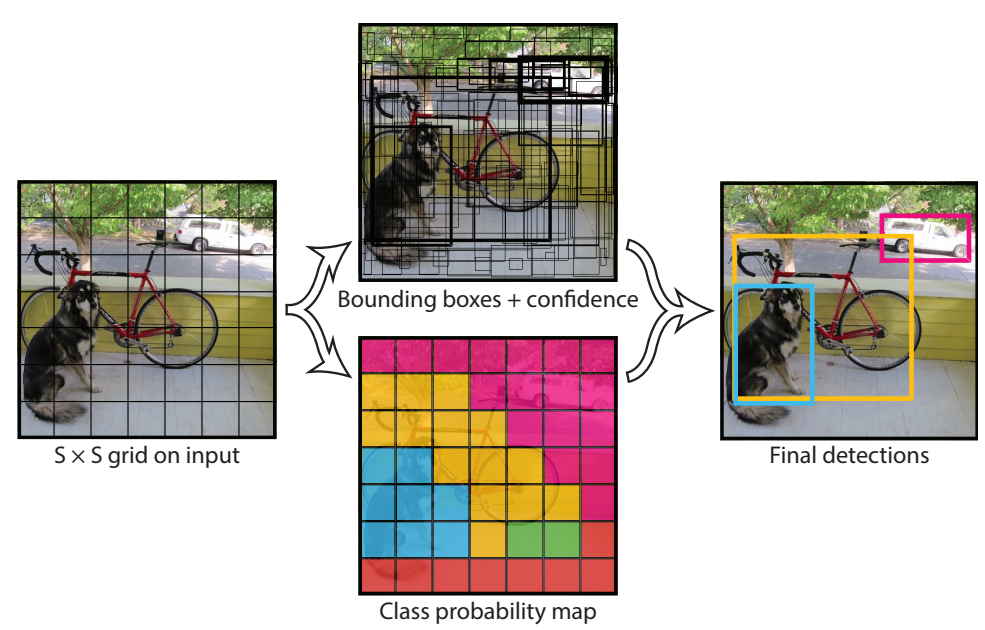
\includegraphics[width = 0.75\textwidth]{./Images/YOLO_stages.PNG} 
\caption{The stages of YOLO. First dives into $S \times S$ grid. Separately predicts bounding boxes with respective confidence, as well as class probability. Then, combines the two to form the final predictions. Image taken from \cite{YOLO1}.}
\label{fig:YOLO_stages}
\end{center}
\end{figure}

Comparisons done by the team working on \textit{YOLO} found that, compared to other real-time systems at the time, both \textit{Fast YOLO} and \textit{YOLO} outperformed them all with \textit{Fast YOLO} being the fastest, but \textit{YOLO} being more accurate on the \textit{PASCAL VOC} data sets \cite{PASCAL}.

Throughout the years Redmon et al. has been working on updating the design pattern of the 
YOLO network. First in 2016 when they introduced \textit{YOLOv2} and then April 2018 with \textit{YOLOv3} \cite{YOLO2}\cite{YOLO3}. \textit{YOLOv2} added a few concepts to the system to make it even more fast and accurate than the earlier iteration. It removed the fully connected layers and is was now possible to train on several different input image resolutions and it could now also predict many more bounding boxes than its predecessor. \textit{YOLOv3} added some changes which improved its ability to detect small objects, with the trade off of having a bit worse performance when finding larger sized objects.  

\subsection{Mean Average Precision}
Metrics for object detection
\url{https://github.com/rafaelpadilla/Object-Detection-Metrics}

mAP (mean Average Precision) for Object Detection
\url{https://medium.com/@jonathan_hui/map-mean-average-precision-for-object-detection-45c121a31173}

The PASCAL Visual Object Classes (VOC) Challenge
\url{http://homepages.inf.ed.ac.uk/ckiw/postscript/ijcv_voc09.pdf}

COCO Detection Evaluation
\url{http://cocodataset.org/#detection-eval}

[VARFÖR INTE "VANLIGA" METRICS?]

[PRECISION]

[RECALL]

[IOU]

\newpage
